\pagestyle{fancy}
\chapter{Localization}
\label{chp:localization}
%\pagenumbering{arabic}
\begin{center}
\textit{This chapter, in particular for the computational evaluation,
is based on the article at Ref. \citen{jcc-26-1042-2005}}
\end{center}
{\ }\\
\vspace{-1mm}

The need to evaluate the properties of large molecular systems using a high-level
\textit{ab initio} approach is an interesting and challenging task for the
quantum chemist. Many useful results have been achieved in this direction,
thanks to refinements of theoretical approaches, together with computational
resources increasingly more efficient and cheap.  However, the problem of
the growth of the computational effort as a function of the system size
still represents, in most cases, a serious bottleneck.  This can lead to a
huge computational cost even for relatively small systems.  

Many techniques have been implemented to deal with large systems, like, for
instance, metallic complexes with organic ligands, or biologically
interesting molecules.  For example, in the evaluation of potential energy
surfaces of the ground state a Molecular Mechanics approach makes feasible
calculations on large molecular systems. The price to pay, in this case, is
to consider the system as purely classical.

When a quantum mechanical evaluation is needed (description of excited states,
bond breaking, etc.), the mixing of molecular mechanics with
quantum mechanics is a possible strategy, like Quantum Mechanics/Molecular
Mechanics QM/MM \cite{jcc-11-700-1990} and the ``Our own N-layered Integrated
molecular Orbital and molecular Mechanics'' ONIOM method
\cite{jpc-100-19357-1996}. For the calculation of excited states,
Time Dependent Density Functional Theory (TDDFT) methods are also
available, which behave well in some cases but with substantial errors in
others, as pointed out for example in Ref. \citen{jacs-126-4007-2004}. 

Performing purely \textit{ab initio} evaluations is also feasible. A
possible approach is represented by the elimination of large molecular
groups, replacing them by computationally cheaper mimicking entities, using
Effective Group Potential (EGP) pseudo-potentials
\cite{jpca-105-198-2001,jpca-105-206-2001}, for example, or simply by
hydrogen atoms. Other available methods, like the Symmetry Adapted
Cluster-Configuration Interaction
(SAC-CI)\cite{jcp-68-2053-1978,cpl-59-362-1978,cpl-67-329-1979,cpl-67-334-1979}
have been applied successfully to large biological systems
\cite{cpl-250-437-1996}.

Another possible strategy in the treatment of large molecular systems is
given by Localized Molecular Orbitals (LMO). The use of localized orbitals in
quantum chemistry has a long history \cite{chavet-ladiqc}.  Only in recent
years, however, Localized Molecular Orbitals have become popular as a key
step toward Linear Scaling \textit{ab initio} approaches, where the
computational cost of the evaluation grows linear with respect to the
molecular system size. Using a localized philosophy, a reduction of the
high computational cost imposed by delocalized methods can be obtained.

\section{Advantages of a localized approach}

In general, delocalization of molecular orbitals is not a physical
requirement. A delocalized picture of the orbitals gained mainstream
attention in connection with the ionization energy as expressed by the
Koopmans theorem. Delocalization can also explain some phenomena in those
systems that possess intrinsic physical delocalization, like for example
polyene chains or aromatic molecules.

However, when a molecule behaves like a set of localized bonds, a
delocalized description introduces a high degree of complexity. As an
example, a localized point of view clearly explains the similar behavior
of C-H bonds in methane, ethane and cyclohexane. A delocalized description
of this physical phenomenon is more difficult.

Delocalization is also a frequent consequence of the mathematical procedures
implemented for orbital optimization. Improving the mathematical asset in
order to obtain spatially localized orbitals allows the quantum chemist to
deal with a more practical representation of the charge distribution, and 
also provides possible new strategies in reducing the computational cost
for \textit{ab initio} evaluations.

A reliable evaluation of the static and dynamic correlation is the main 
limiting factor for a quantum chemical approach to medium and large
molecular system. These contributions to the energy are critical, and their
evaluation computationally demanding, but their nature is a local
phenomenon, related to the spatial distribution of the electrons. A
delocalized approach imposes very expensive evaluations: the physical effect
of correlation is spread over a large number of integrals. Each of these
integrals accounts for an almost unpredictable quantity to the energy, and
their physical meaning is difficult to understand.

Making use of a localized description, interactions between electrons
populating distant, non-overlapping orbitals can be considered negligible, and
thus candidate for being eliminated from the evaluation. As a direct
consequence, correlative effect are now concentrated on a reduced set of
highly important integrals. Neglecting these long-range interactions due to
locality of the molecular orbitals is an important strategy to reduce the
computational cost.

Linear Scaling techniques are already available for SCF calculations
\cite{rmp-71-1085-1999}, M{\o}ller-Plesset perturbative treatments (MP) at
different orders
\cite{jcp-110-3660-1999,pulay-gdesmp,jcc-19-1241-1998,cpl-290-143-1998,
tca-69-357-1986,jcp-86-914-1987,ijqc-70-167-1998}
Single and Double Configuration Interaction (SDCI) \cite{jcp-104-6286-1996},
Single and Double
Coupled Cluster (CCSD)\cite{jcp-104-6286-1996,jcp-111-8330-1999}
and CCSD(T)\cite{jcp-113-9986-2000,jcp-114-661-2001}.  All the cited methods
apply to a single reference wavefunction, and are therefore unbalanced when
two or more determinants of nearly equal weight are critical in the
description of the system. % FIXME ripete il concetto in alto ?
Although multireference Linear Scaling techniques
are still to be devised, a localized orbitals approach is recognized as an
important requisite in achieving this objective, allowing a ``\textit{divide et
impera}'' strategy on the molecule.

It is important to note that many chemically interesting problems require
the application of a multireference scheme in order to produce reliable
results.  Examples of these problems are the treatment of bond breakings,
electronically excited states, magnetic systems, and charge transfer.
Treatment of these systems is important to gather a deep insight in
biological catalysis, photochemical reactions, high atmosphere degradation
of polluting compounds, technological improvements for data storage, data
transfer and computation. 

Localization of molecular orbitals can also benefit multireference
evaluations in terms of quality and size of the active space. 
Phenomena involving electronic excitation or bond breaking usually happen in a
well localized region of the molecule. 

Working with delocalized orbitals, the active space needed to describe these
phenomena is normally defined by those MOs bringing the highest correlative
effects, regardless of the spatial or physical nature. Moreover, the user
has poor or no control of the active orbital selection. Using local
orbitals, a well defined and physically clear active space can be chosen and
maintained during the optimization. 

Finally, a reduction of the reference space can also be obtained: a
localized description clearly depicts which determinants are not important
for the description of the wavefunction, because they express highly ionic
electronic distributions where a large number of electrons are concentrated
in a certain region of space. 

\section{Existent methods of localization}

In the past, localized orbitals describing the molecule were obtained
performing an appropriate transformation of a delocalized manifold, i.e.
applying a unitary transformation to the spatial orbitals row vector
$\mathbf{\psi}$
\beq
\mathbf{\psi}_{\mbox{\tiny loc}} = \mathbf{\psi}_{\mbox{\tiny deloc}} \mathbf{U}
\eeq

Finding localized, equivalent orbitals is normally achieved choosing a
$\mathbf{U}$ matrix which maximizes a ``localization function''.
For example, the contribution from Edmiston and Ruedenberg
\cite{rmp-34-457-1963} aims at minimizing the Coulomb repulsion between
electron pairs occupying two different orbitals.  If $\phi_i$ and $\phi_j$
are two different orbitals, then satisfying the condition
\beq
\sum_{i<j}^{\mbox{\tiny occ}} \braket{\phi_{i}\phi_{j}}{g}{\phi_{i}\phi_{j}} = \mbox{minimum}
\eeq
imposes locality of the charge distribution.  Another approach from
Boys\cite{rmp-32-2-1960} is to maximize the distance between the centroids
of the transformed orbitals.  Other methods, like for example those by
Pipek\cite{jcp-90-4916-1989}, Angeli et al.\cite{cpl-233-102-1995} work
along the same principle, and can be classified as \textit{intrinsic
methods} of localizations.  \textit{Extrinsic methods} work equally well,
and they are realized performing a projection of localized MO's onto a
delocalized optimized manifold\cite{chavet-ladiqc}. 

All these methods resort on \textit{a posteriori} localization techniques,
therefore a prior evaluation of delocalized canonical MOs is needed.
Obtaining a localized set of orbitals is also possible using \textit{a
priori} methods, where a controlled optimization procedure is applied on a
localized but unoptimized guess of orbitals.  The controlled procedure
preserves the locality, rather than imposing it. Methods that address SCF
equations already exist\cite{jcp-34-89-1961,prl-4-17-1969,gilbert-moicpb}.

The main advantage of an \textit{a priori} method is the possibility to
choose and preserve the nature of the active space during a CAS evaluations.
This property is of particular importance in order to build a CAS space
using the orbitals involved in the chemical or physical process under study.

In all these methods, the local orbitals are expressed as an orthogonal set.
In general this approach is computationally more efficient compared to
Generalized Valence Bond methods\cite{jcp-57-738-1972,bobrowicz-mest}
where a set of non-orthogonal orbitals with atomic character is
variationally optimized.


\section{Toulouse method of localization}
\label{sec:toulouse_method}

An \textit{a priori} localization method has been recently proposed by the
working group in Toulouse, with the goal to address multireference problems. 
The method has been applied to the description of the excited
state of polyenes polyenals, polyendials and polyenones
\cite{ijqc-101-325-2005,ijqc-97-688-2004,cpl-372-22-2003,mp-101-1389-2003},
C$_{60}$ Fullerene + Sodium interaction \cite{jms_theo-681-203-2004}, nickel
and copper chains \cite{cpl-378-503-2003} in a mixed localized/delocalized
approach, Cu magnetic systems \cite{jpca-107-7581-2003}, Hydrogen chains
\cite{jms_theo-621-51-2003}, and Mo-Cl complexes \cite{cpl-349-555-2001}.

Briefly, this method preserves the local character of LMO, converging to a
CASSCF wavefunction. A localized guess is obtained through the projection
of Localized Molecular Orbitals (LMO) onto the delocalized SCF manifold.
Then, the locality is preserved avoiding a complete diagonalization of the
density matrix. 

Three versions of the optimization algorithm are currently available: 
a variational uncontracted \cite{jcp-116-10060-2002}, developed in Toulouse,
a perturbative contracted \cite{jcp-117-10525-2002} and the recently deployed
variational contracted, both developed in Ferrara.

The subsequent work is based on the variational uncontracted approach. This
approach does not converge to a rigorous CASSCF solution, because of the
uncontracted nature of the implemented CI expansion.  However, as already
shown in Ref. \citen{jcp-116-10060-2002}, this fact does not seem to
have severe practical effects.

\subsection*{Creation of the guess}

The method starts with the creation of a set of Orthogonal Atomic Orbitals
(OAO), obtained through a Schmidt orthogonalization and a $S^{-\frac{1}{2}}$
normalization of the atomic basis set. ANO type \cite{tca-77-291-1990} is
preferred, since the orbitals are described by a minimal number of coefficients.

The orthonormalization is performed against a hierarchical classification of
the orbitals: the core orbitals are orthogonalized among themselves, then
the valence orbitals against the cores and among themselves, finally the
remaining orbitals. The obtained OAOs are then used to build Localized
Molecular Orbitals (LMOs) as linear combinations of OAOs, using the
one-electron density matrix of a one-electron evaluation (Huckel or SCF):
\beq
R_{ij} = \braket{\Phi_{0}}{a_i^+ a_j}{\Phi_{0}}
\eeq

It is possible to define a projector for an atom K (built using the projector onto
the $\tilde{\chi}_{l}$ OAO functions) or for a molecular fragment F (from a sum of projectors
onto the involved atoms)
\beqa
P_{K} = \sum_{l \in K} \ket{\tilde{\chi}_{l}} \bra{\tilde{\chi}_{l}} \\
P_{F} = \sum_{K \in F} P_{K}
\eeqa

The density matrix obtained by the projected wavefunction $P_{F}
\Phi_{0}$ can be diagonalized. This step leads to a linear combination of
OAO, representing MO's localized on the fragment. Some of these MO's
exhibit occupation numbers which are close to two or zero, and they
represent a localized bond between the atoms involved in the fragment. Other
orbitals can exhibit occupation numbers close to one, and they are rejected
since they are hybrid orbitals that are representative of an ``half-bond''
between non considered atoms.

As an example, the creation of LMO's in the carbonyl group of acetone is
here presented.

{\small
\begin{verbatim}
Extracted matrix
----------------

O1 1s   1.6881  0.0000  0.0000  0.3780  0.2764  0.0000  0.0000  0.5185
O1 2px  0.0000  1.2406  0.0000  0.0000  0.0000  0.9340  0.0000  0.0000
O1 2py  0.0000  0.0000  1.8980  0.0000  0.0000  0.0000  0.2703  0.0000
O1 2pz  0.3780  0.0000  0.0000  1.4621 -0.4912  0.0000  0.0000 -0.6081
C1 1s   0.2764  0.0000  0.0000 -0.4912  0.9477  0.0000  0.0000 -0.0968
C1 2px  0.0000  0.9340  0.0000  0.0000  0.0000  0.8168  0.0000  0.0000
C1 2py  0.0000  0.0000  0.2703  0.0000  0.0000  0.0000  1.0402  0.0000
C1 2pz  0.5185  0.0000  0.0000 -0.6081 -0.0968  0.0000  0.0000  0.9164

Orbitals
--------
 
Occup.
Number  1.9975  1.9865  1.9777  1.9761  1.0201  0.9622  0.0709  0.0190
  
O1 1s  -0.5478  0.0000  0.7384  0.0000 -0.0855  0.0000  0.0000 -0.3838
O1 2px  0.0000  0.7814  0.0000  0.0000  0.0000  0.0000 -0.6240  0.0000
O1 2py  0.0000  0.0000  0.0000  0.9607  0.0000 -0.2775  0.0000  0.0000
O1 2pz  0.5405  0.0000  0.6639  0.0000 -0.0413  0.0000  0.0000  0.5151
C1 1s  -0.3477  0.0000 -0.1176  0.0000 -0.8134  0.0000  0.0000  0.4512
C1 2px  0.0000  0.6240  0.0000  0.0000  0.0000  0.0000  0.7814  0.0000
C1 2py  0.0000  0.0000  0.0000  0.2775  0.0000  0.9607  0.0000  0.0000
C1 2pz -0.5356  0.0000 -0.0089  0.0000  0.5739  0.0000  0.0000  0.6195

----------------------------------------------------------------------
    Occupied               Eliminated             Virtuals
 1.9975... 1.9761 /  /  1.0201...  0.9622 /  /  0.0709 ... 0.0190
\end{verbatim}

}

As can be seen, the extracted density matrix leads to a localized set of
orbitals. The first four, with occupation numbers close to two, are the
C-O $\sigma$ bond, the CO $\pi$ bond, and the lone pairs $n_z$ and $n_y$.
Two orbitals express the half $\sigma$ bonds directed toward the remaining
carbon atoms. These bonds will be kept into account in other selections, so
they are discarded. Finally, two orbitals with occupation number close to
zero express the C-O $\pi^{*}$ and $\sigma^{*}$.  The resulting set of LMOs
is not orthogonal, so a new hierarchical orthonormalization is performed.

The obtained orbitals are then projected onto a delocalized SCF manifold.
This step, like an extrinsic method of localization, provides a localized
SCF-quality set of orbitals.

\subsection*{Optimization of the guess}

In the classical (non Freeze-and-Cut) localization technique, orbitals
obtained from the last step are then optimized at CASSCF level.  Working on
a single reference SCF wavefunction $\Phi_{0}$, the optimization
should follow these steps:
\begin{enumerate}
\item define a single excitation configuration interaction
$\Psi_{\mbox{\tiny CIS}} = \Phi_{0} + \sum_{i,r} C_{ir} a_{r}^{+} a_i \Phi_{0}$
and obtain the $C_{ir}$ coefficients through diagonalization
\item create the one electron density matrix $R_{ir} =
\braket{\Psi_{\mbox{\tiny CIS}}}{a_{r}^{+} a_i}{\Psi_{\mbox{\tiny CIS}}}$ and
block diagonalize it
\item use the new set of orbitals to create a new $\Phi_{0}$, and iterate until
$\Psi_{\mbox{\tiny CIS}} = \Phi_{0}$, satisfying the Brillouin theorem \cite{asi-159-1934}.
\end{enumerate}

Particular care must be applied in the density matrix diagonalization step.
A complete diagonalization leads to delocalized natural orbitals. To prevent
this behavior, a controlled block diagonalization is performed
\beq
R_{\mbox{DP}} = W^{+} R W
\eeq
where $R$ is the density matrix, $R_{\mbox{\tiny DP}}$ is the block diagonalized
density matrix, and $W$ is a unitary matrix, given by
\beq
W = U_{\mbox{\tiny D}} U_{\mbox{\tiny P}}^{+}
\eeq
where $U_{\mbox{\tiny D}}$ is a matrix that fully diagonalizes $R$ and
$U_{\mbox{\tiny P}}$ is a matrix that restores the orbital locality, mixing those
orbitals inside the same class (occupied or virtual, in the case of
a single reference calculation). The $U_{\mbox{\tiny P}}$ matrix is obtained
through projection of $U_{\mbox{\tiny D}}$ onto the subspaces and a subsequent
orthonormalization.

The same working principle can be applied to multireference CAS
wavefunctions: using a CAS space, the CI energy and wavefunction are
invariant with respect to rotations inside each block of core, active
and virtual orbitals. This invariance allows us to produce localized orbitals
equivalent to the delocalized ones, and locality can be maintained
preventing as much as possible rotations inside each of the three blocks.

The requirement for convergence is to satisfy the Extended Brillouin Theorem
\beq
\braket{\Psi_{\mbox{\tiny CASSCF}}}{\ham \left[ a_{k}^{+} a_{l} -
a_{l}^{+} a_{k} \right]}{\Psi_{\mbox{\tiny CASSCF}}} = 0
\eeq
which is always fulfilled if $k$ and $l$ refer both to core, active or
virtual orbitals. The previous equation can threfore be decomposed in three
equations between different classes of indexes:
\beqa
\braket{\Psi_{\mbox{\tiny CASSCF}}}{\ham \left[ a_{a}^{+} a_{i} -
a_{i}^{+} a_{a} \right]}{\Psi_{\mbox{\tiny CASSCF}}} & = & 0 \\
\braket{\Psi_{\mbox{\tiny CASSCF}}}{\ham \left[ a_{r}^{+} a_{i} -
a_{i}^{+} a_{r} \right]}{\Psi_{\mbox{\tiny CASSCF}}} & = & 0 \\
\braket{\Psi_{\mbox{\tiny CASSCF}}}{\ham \left[ a_{r}^{+} a_{a} -
a_{a}^{+} a_{r} \right]}{\Psi_{\mbox{\tiny CASSCF}}} & = & 0
\eeqa
where $i$, $a$ and $r$ refer to core, active and virtual orbitals,
respectively. In order to minimize the energy, the non-interaction of
singly-excited contracted CAS wavefunctions must be reached iteratively
using the Super-CI approach. A prototype for this approach has been
developed in Ferrara laboratory, and has been used for the combined
Localization-NEVPT2 evaluation, presented later in this thesis.

An alternative solution, followed at Toulouse laboratories, is to consider a
decontracted scheme, exploiting the full dimensionality defined by the space
of determinants $S = \{\Phi_i\} \cup \{a^{+}_{r} a_{i} \Phi_i\}$ spanned by
the CAS space and their single excitations. The procedure is not a Super-CI
optimization and does not converge to the real CASSCF solution. However, as
pointed out in Ref. \citen{jcp-116-10060-2002}, the resulting orbitals
are very similar to the CASSCF ones.

The third possibility is to work with a perturbartive contracted approach.
The idea is to consider the $\Psi_{\mbox{\tiny CASCI}}$ at a given iteration as a
zero-order description of the $\Psi_{\mbox{\tiny CAS+S}}$. We diagonalize a
zero-order Hamiltonian inside a perturber space Q, spanned by the singly
excited contracted functions $a_{a}^{+} a_{i} \ket{\Psi_{\mbox{\tiny CASCI}}}$,
$a_{r}^{+} a_{i} \ket{\Psi_{\mbox{\tiny CASCI}}}$ and $a_{r}^{+} a_{a}
\ket{\Psi_{\mbox{\tiny CASCI}}}$. From the diagonalization, we obtain perturber
wavefunctions as linear combinations
\beq
\ket{\Psi_{\mu}} = \sum_{ai} c_{ai \mu} \constr{a} \destr{i}
\ket{\Psi_{\mbox{\tiny CASCI}}} + \sum_{ri} c_{ri \mu} \constr{r} \destr{i}
\ket{\Psi_{\mbox{\tiny CASCI}}} + \sum_{ra} c_{ra \mu} \constr{r} \destr{a}
\ket{\Psi_{\mbox{\tiny CASCI}}}
\eeq
and the first-order correction to the wavefunction is
\beq
\ket{\Psi^{(1)}} = \sum_{\mu}
\frac{\braket{\Psi_{\mu}}{\ham}{\Psi_{\mbox{\tiny CASCI}}}}{E_{\mbox{\tiny CASCI}}-E_{\mu}^{(0)}}
\ket{\Psi_{\mu}}
\eeq
From this correction, it is possible to obtain the correction to the
one-particle density matrix
\beqa
\rho_{lk}^{(1)} & = & \sum_{\mu} \left\{
\frac{\braket{\Psi_{\mbox{\tiny CASCI}}}{a_{k}^{+} a_{l}}{\Psi_{\mu}}
\braket{\Psi_{\mu}}{\ham}{\Psi_{\mbox{\tiny CASCI}}}}{E_{\mbox{\tiny CASCI}}-E_{\mu}^{(0)}}
+ \right. \nonumber \\
& & \left. + \frac{\braket{\Psi_{\mbox{\tiny CASCI}}}{\ham}{\Psi_{\mu}} \braket{\Psi_{\mu}}{a_{k}^{+}
a_{l}}{\Psi_{\mbox{\tiny CASCI}}}}{E_{\mbox{\tiny CASCI}}-E_{\mu}^{(0)}} \right\} 
\eeqa
When the convergence is reached, the correction vanishes.
For the choice of the zero-order Hamiltonian, is convenient to make use of a
particular Hamiltonian, the Dyall's Hamiltonian\cite{jcp-102-4909-1995}
\beqa
\ham^D &=& \ham^D_i + \ham^D_v + C \\
\ham^D_i &=& \sumidx{i} \epsilon_i \constr{i} \destr{i} + \sumidx{r}
\epsilon_r \constr{r} \destr{r} \\
\ham^D_v &=& \sumidx{ab} h_{ab}^{\mbox{\tiny eff}} \constr{a} \destr{b} +
\frac{1}{2} \sumidx{abcd} \integral{ab}{cd} \constr{a}\constr{b}
\destr{d}\destr{c}
\eeqa
where labels $i,j,\ldots$, $a,b,\ldots$, $r,s,\ldots$ denote core, active and
virtual orbitals respectively, and $ h_{ab}^{\mbox{\tiny eff}} =
\braket{a}{h+\sumidx{i}\left( J_i - K_i \right)}{b}$.
This Hamiltonian, which will be presented in more details in the n-Electron
Valence state Perturbation Theory approach, leads to a simplification of the
computational asset. The zero-order Hamiltonian is defined as the projection
of the Dyall inside the interested spaces
\beq
\ham_{0} = \proj{\mbox{\tiny CAS}} \ham^D \proj{\mbox{\tiny CAS}} +
\proj{\mbox{\tiny Q}} \ham^D \proj{\mbox{\tiny Q}}
\eeq
The perturbative approach is very straightforward and efficient, and
converges to the real CASSCF wavefunction. However, divergent behaviors 
have been reported when the zero-order wavefunction needs a strong
correction.



\section{Freeze-and-Cut method}

A fundamental assumption in reducing the computational cost of
\textit{ab initio} evaluations is that correlative effects are usually local,
given the nature of the studied phenomena.
For this reason, the molecular framework not involved in chemical or
physical phenomena is an ideal candidate to be frozen at a lower level of
theory, like for example SCF, after the creation of the localized guess.
This strategy has already proved its efficiency in reducing the computational
cost \cite{jms_theo-681-203-2004}, but has no influence on the basis set
size, only the number of molecular orbitals. This is a particularly
severe limitation for MRCI methods, which require a two-electron AO/MO
integral transformation for all correlated orbitals.  This step grows as
$N_{\mbox{\tiny AO}}^4 N_{\mbox{\tiny MO}}$, where $N_{\mbox{\tiny AO}}$ is the number of
Atomic Orbitals (AO) and $N_{\mbox{\tiny MO}}$ is the number of Molecular
Orbitals (MO). If no freezing is performed on the molecular orbitals, the
transformation grows as $N^5$. Freezing a part of the orbital set a
rectangular transformation is performed and the computational
weight is reduced, but the quartic dependence on $N_{\mbox{\tiny AO}}$ still
limits calculations on large AO spaces. This problem must be managed in
order to perform calculations with a reduced dependency of the basis set.

A possible strategy is to cut out the molecular framework that is not
essential for the description of the phenomenon under study.  In other
words, \textit{all the atoms whose AOs are not fundamental in the description
of the non-frozen MOs are eliminated}. The subsequent CASSCF optimization is
performed in the preserved molecular framework only, \textit{under the
effect of the eliminated nuclei and electrons as provided by the freeze}.
This effect takes into account sterical interaction and charge effects
provided by the frozen framework internally (within itself) and externally
(onto the non-frozen framework), given that the AO/MO transformation of the
integrals retains information about the frozen framework.

Moreover, once the CASSCF optimization has been performed, the method
leaves freedom for application of higher levels of theory, still preserving
the effects of the frozen molecular framework at a lower level of theory.

\subsection*{Computational procedure}

The procedure starts with the creation of a set of SCF delocalized orbitals,
which is subsequently localized to obtain a localized SCF set. The resulting
localized orbitals, each one mainly described on a reduced set of atomic functions, are
selected for the freezing step. The remaining unfrozen orbitals are then
projected onto a reduced AO space, setting to zero the coefficients on
those AOs that are not essential for the expression of the orbitals.

\begin{figure}[ht]
\begin{center}
\includegraphics[width=7cm,keepaspectratio]{02_localization/images/matrix.eps}
\caption{\footnotesize A visual representation of large (ORTORBL) and small (ORTORBS)
molecular orbitals matrices. Localized orbitals are first classified as frozen or
non-frozen. The non-frozen orbitals are supposed to have negligible
coefficients on distant atoms. These coefficients are strictly set to
zero by the cut procedure, and a localized optimization is performed in the
obtained AO/MO subspace. }
\label{fig:matrix}
\end{center}
\end{figure}



This procedure leads to two different orbital matrixes. The first one
has the dimension of the original AO basis set, but with some of
the coefficients of non-frozen orbitals set to zero. The second one is
the submatrix of coefficients that belong to unfrozen orbitals
(see Fig. \ref{fig:matrix}).  The latter has a reduced dimension, and
corresponds to the effective space on which the optimization procedure will
be performed.

The orbitals from the two matrixes are no longer orthogonal, and a
hierarchical orthonormalization is performed on the large matrix (non-frozen
orbitals first, then frozen orbitals against the non-frozen ones) and on the
small matrix, to obtain two sets of orbitals, named ORTORBL and ORTORBS
respectively.  An AO/MO integral transformation is performed at each
iteration from the improved orbitals. One-electron MO integrals are provided
by the full dimensional orbital structure, while two-electron MO integrals
are evaluated only on the reduced set described by ORTORBS. 

This procedure results in a spatial confinement of the non-frozen orbitals,
improving the ORTORBS orbitals only inside this reduced AO space. These MOs
have strictly zero coefficients on any AO belonging to the eliminated
region.  For this reason, the method is affected by the truncation of
orthogonalization tails for large basis sets, or in the case of highly
delocalized systems. In general this truncation affects the absolute
energies, with very little effect on the energy differences.

The computational chain is built to interface \molcas 5.4 \cite{molcas-site}, with
a set of small home-developed softwares and bash scripting in GNU/Linux
\cite{gnu-linux-site} environment to provide the complete deployment of this
technique.

A scheme for the method is depicted in Fig. \ref{fig:logical-scheme}.
The scheme focuses on the results (depicted as boxes) obtained through processing steps
(depicted as arrow lines). Thick arrows represent processes that involves evaluation or
use of integrals on the complete system and so represent still a bottleneck
in this technique. Improvements are planned to skip this evaluation, by making
use of a direct SCF procedure.
The formalism can be subdivided into two logical steps:
\begin{itemize}
\item creation of the localized guess (upper part of the scheme)
\item iterative optimization of the localized guess (lower part, enclosed
into dashed frame)
\end{itemize}
The upper part of the scheme can also be subdivided in two independent
calculations: the large calculation, performed on the complete molecular
geometry (left side of Fig. \ref{fig:logical-scheme}) and the small calculation,
performed only on the geometry resulting after the cut operation (truncated
system, right side of Fig. \ref{fig:logical-scheme}).  The localized guess
is obtained through the following strategy:
\begin{itemize}
\item evaluation of the AO integrals on the large system, by using standard
software components from the \molcas 5.4 package
\item calculation of delocalized SCF orbitals
\item creation of a localized guess that describes the bonds or the groups we are
interested in
\item projection of the localized guess onto the SCF delocalized orbitals
\end{itemize}

\begin{figure}[h!]
\begin{center}
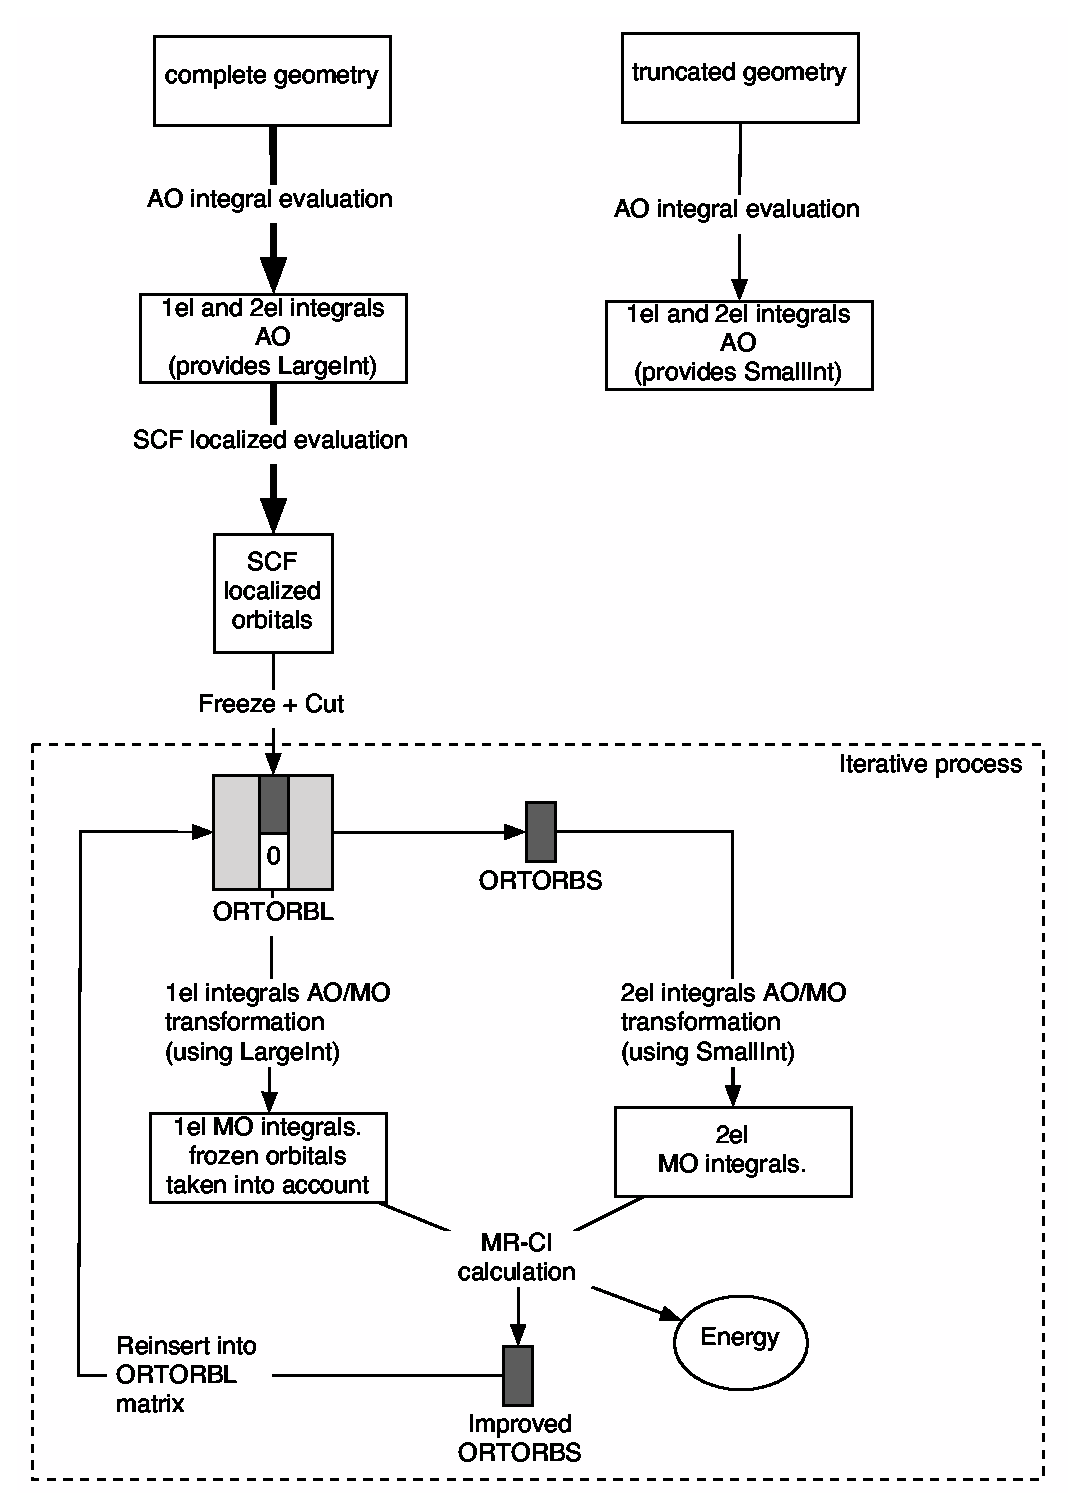
\includegraphics[width=13cm,keepaspectratio]{02_localization/images/logical-scheme-gimped.eps}
\caption{\footnotesize Logical steps (arrows) and obtained entities (boxes) for the
presented procedure. Thick lines denote steps that still depend on two
electron AO integrals on the complete geometry of the system
} \label{fig:logical-scheme}
\end{center}
\end{figure}


These steps describe in more detail the process labeled 
as ``SCF localized evaluation'' in Fig.~\ref{fig:logical-scheme}. The result
is a set of orthogonal localized SCF orbitals.

Thanks to the localization procedure, each localized SCF orbital is mainly
described on a reduced set of atomic basis functions. These orbitals can now
be tagged on two degrees of freedom: the freezing selection of certain
localized SCF orbitals, and the cut of a set of atomic basis functions for
the non-frozen orbitals. The latter is realized by setting to zero the
coefficients that express the non-frozen orbitals on the cut atomic basis
set. This operation effectively projects the non-frozen MO in a reduced
atomic basis space, and the approximation is good as long as the target
coefficients are already close to zero due to the localization.

The large MO matrix (refer to the detailed pictorial representation in
Fig.~\ref{fig:matrix}) holds molecular orbitals that are no longer
orthonormal, although it must be pointed out that the overlap between them
is small. A hierarchical orthonormalization is performed to obtain an
orthonormal set: first the non-frozen orbitals among themselves, then the
frozen occupied orbitals with respect the non-frozen, and finally the frozen
virtual orbitals. Thanks to the hierarchical procedure, the coefficients
that have been set to zero remain unchanged. This is important in order to
keep the non-frozen orbitals inside a smaller AO space.

Finally, a smaller matrix is obtained by extracting the submatrix
of the non-frozen orbitals against the smaller, non-cut atomic set.
The final result of this process are two matrixes, named ORTORBL and
ORTORBS, which hold the molecular orbitals as described, respectively for
the large and the small system (complete system and truncated one).

After an AO/MO integral transformation, the optimization chain is now fed
with two-electron MO integrals (which derive only from orbitals
that are not frozen) and with the modified one-electron integrals that keep
into account the two-electron contribution from the frozen set. 

At each iteration, the procedure works as follows:
\begin{itemize}
\item calculate an improved density matrix using a Super-CI
optimization that preserves orbitals locality. This process is
done only on the restricted subset of non-frozen orbitals, and only on the
available framework of non-cut atoms, leading to an improved set
of orbitals (improved ORTORBS)
\item reinsert the improved orbitals inside the frozen framework, thus creating
an improved ORTORBL large matrix
\item recreate a new set of MO two-electron integrals, transforming the AO integrals
from the truncated system using the improved ORTORBS orbitals
\item recreate a new set of MO one-electron integrals with the improved ORTORBL set
and the complete system
\item iterate until convergence is reached (no change in the energy within a
given level of approximation)
\end{itemize}

\input{02_localization/04_freeze_and_cut_implementation}
\pagebreak
\section{Evaluations}
\subsection{(7Z)-13 ammoniotridec-7-enoate}

The first test case presented is relative to (7Z)-13 ammoniotridec-7-enoate, an
aminoacid zwitterion specifically designed to test the response of the
method to charge interactions (see Fig. \ref{fig:7Z-molecule}). The rigid
rotational behavior around the central double bond has been evaluated,
describing the absolute CAS+Single excitations (CAS+S) energy curves without
geometry relaxation with respect to the torsional dihedral angle. 

\begin{figure}[ht]
\begin{center}

\includegraphics[width=7cm,keepaspectratio]{02_localization/images/7Z-molecule.eps}
\caption{\footnotesize The (7Z)-13 ammoniotridec-7-enoate molecule. The cis-trans rigid
interconversion around the central double bond has been performed to test
the presented method. }
\label{fig:7Z-molecule}
\end{center}
\end{figure}



All the calculations have been performed by using ANO basis sets.
A minimal basis set ANO-1\cite{tca-77-291-1990} with
$2s1p$ contraction for C,N,O and $1s$ contraction for hydrogen atoms was
used.  The interatomic distances (in $\mbox{{\AA}ngstrom}$) are
r(C-C)=1.450, r(C=C)=1.335, r(C-H)=1.089, r(C-N)=1.440, r(N-H)=1.008,
r(C-O)=1.400. The angles are 109.5 degrees except for the C=C group and the
COO$^{-}$ group, where angles of 120 degrees have been used.
The dihedral angles were adjusted to obtain the cis and trans molecular
skeleton lying completely on the plane.

The CAS space selection consists of 2 electrons in 2 orbitals (C-C $\pi$
and $\pi^{*}$). This selection has been chosen to keep into account the
main correlative effects due to the rotation around the central
carbon-carbon double bond.

It must be stressed that, due to geometrical proximity, the interaction
between the charged groups affects the rotational behavior, and its
contribution must be kept into account.  For this reason, the two terminal groups
cannot be simply removed and replaced by hydrogen atoms.
As a comparison example, Fig.~\ref{fig:7Z-nocharges} shows the
behavior obtained by removing these groups and replacing them with
hydrogens. 

\begin{figure}[t]
\begin{center}
\includegraphics[width=8cm,angle=270]{02_localization/images/7Z-nocharges.eps}
\caption{\footnotesize A comparison of the CAS+S energy curves between the zwitterionic
(7Z)-13 ammoniotridec-7-enoate (solid line) and the (6Z)-dodec-6-ene, a
molecule obtained by replacing the charged NH$_{3}$ and COO$^{-}$ groups
with hydrogen atoms, dashed line.  A common zero in the energy scale of the
plot has been obtained taking the trans form as zero of the energy.  }
\label{fig:7Z-nocharges}
\end{center}
\end{figure}


Using the Freeze-and-Cut technique, the evaluation performed on a
small system reproduces the expected behavior: the freezing preserves the
electronic contribution of the groups, and the cut allows to work with a
reduced molecular system.

\begin{figure}[h!]
\begin{center}
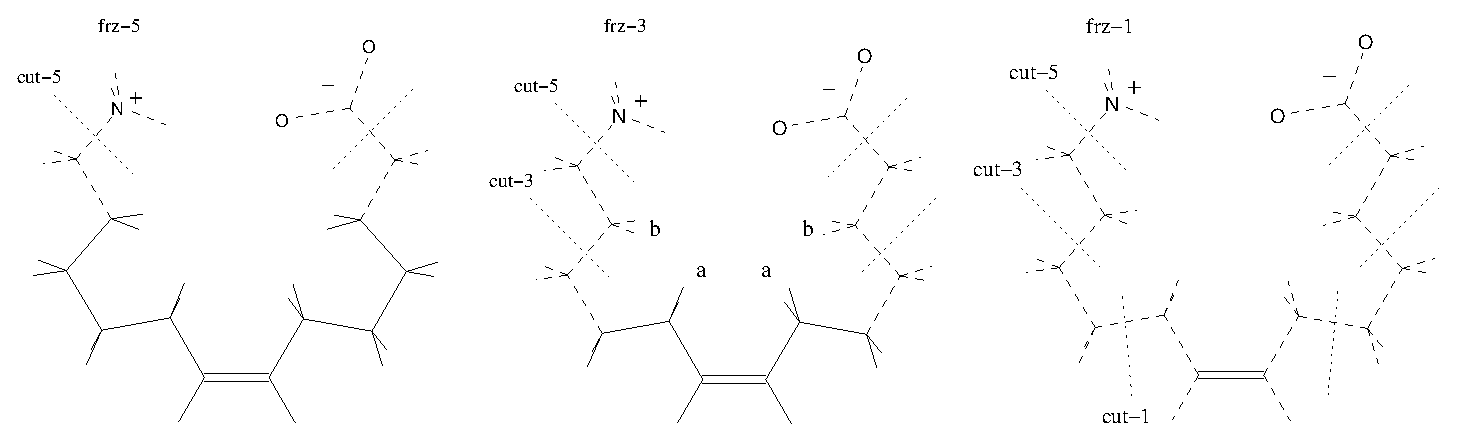
\includegraphics[width=12cm,keepaspectratio]{02_localization/images/7Z-frzcut-schema.eps}
\caption{\footnotesize (7Z)-13 ammoniotridec-7-enoate. Localized orbitals expressed on
atoms of the dashed line framework are frozen. Orbitals expressed on atoms
of the solid line framework are not frozen. Dotted lines depict the
cut seam. The cut is always performed on both chains, from ``cut-5'' (only
the charged groups are removed from the molecule, both left and right) to
``cut-1'' (maximal cut selection, only the central double bond and left and
right -CH$_{2}$- spacers are preserved). The ``a'' and ``b'' symbols in frz-3 picture
are labels for interesting hydrogen atoms. See text for details.  }
\label{fig:7Z-frzcut-schema}
\end{center}
\end{figure}


Different freeze and cut strategies have been chosen in order to evaluate
the behavior of our technique with respect to these selections.
Three freezing levels, labeled ``frz-1,'' ``frz-3'' and ``frz-5'' have been
defined (Fig. \ref{fig:7Z-frzcut-schema}), and also a ``nofrz'' level
where no freezing has been performed.  The $1s$ core atomic orbitals for heavy
atoms have been frozen at SCF level regardless of the atom positions.

The cut strategy follows the freezing strategy. Four cut thresholds have
been chosen, with labels ``cut-1,'' ``cut-3,'' ``cut-5'' and ``nocut,''
following the freezing choice, but preserving a -CH$_2$-
spacer between the last not frozen orbital and the first cutout atom.

The analysis performed at 0 (cis) and 180 (trans) degrees and their
difference are presented in Tab. \ref{tbl:7Z-cis-trans-diff}

\begin{center}
\begin{threeparttable}
\begin{tabular}{lcccc}
\hline
    		&		nofrz			&	frz-5				&	frz-3				&	frz-1	\\	
\hline
			&	\multicolumn{4}{c}{Cis} \\
nocut		&	-709.483006     	&	-709.482889     	&	-709.482281     	&	-709.465687      \\
cut-5		&						&	-709.373507  		&   -709.479395  		&	-709.465638      \\
cut-3		&						&						&	-709.218388     	&	-709.460918      \\
cut-1		&						&						&						&	-709.357068    	 \\
			&	\multicolumn{4}{c}{Trans} \\
nocut		&	-709.388878     	&	-709.388760     	&	-709.388156     	&	-709.371500      \\
cut-5		&						&	-709.279814  		&   -709.385430  		&	-709.371437      \\
cut-3		&						&						&	-709.123318     	&	-709.366578      \\
cut-1		&						&						&						&	-709.258750    	 \\
			&	\multicolumn{4}{c}{Diff} \\
nocut		&	59.0267         	&	59.0272         	&	59.0251         	&	59.0640        	 \\
cut-5		&						&	58.7538         	&	58.9248         	&	59.0725          \\
cut-3		&						&						&	59.6173         	&	59.1598          \\
cut-1		&						&						&						&	61.6542        	 \\
\hline
\end{tabular}
\caption{\footnotesize CAS+S absolute energies (Hartree) and energy
difference (kcal/mol) between (7Z)-13 ammoniotridec-7-enoate cis and trans
structure, with respect to different freeze and cut strategies.}
\label{tbl:7Z-cis-trans-diff}
\end{threeparttable}
\end{center}


It can be seen that the cut technique produces energy differences between
cis and trans that are comparable to the reference value obtained with no
cut and freeze.

A different behavior can be evaluated for the difference between the 0 degrees
form and the 90 degrees form (Tab. \ref{tbl:7Z-diff-cis-90})

\begin{center}
\begin{threeparttable}
\begin{tabular}{lcccc}
\hline
			&		nofrz			&	frz-5				&	frz-3				&	frz-1	\\
\hline
nocut		&	130.4145        	&	130.4953        	&	131.2643        	&	167.4817         \\
cut-5		&						&	130.1703        	&	131.1572        	&	167.5065         \\
cut-3		&						&						&	130.8074        	&	168.4879         \\
cut-1		&						&						&						&	171.2689       	\\
\hline
\end{tabular}
\caption{\footnotesize CAS+S energy difference (kcal/mol) between the (7Z)-13
ammoniotridec-7-enoate cis and the 90 degrees twisted structure with respect
to different freeze and cut strategies.}
\label{tbl:7Z-diff-cis-90}
\end{threeparttable}
\end{center}


The frz-1 selection presents a large deviation from the expected value. This
arises from the fact that the SCF at 90 degrees evaluates very poorly the
orbitals involved (directly or indirectly) in the bond breaking. 

This leads to an initial bad description of the orbitals, which are frozen
at this poor quality level. As a consequence, the optimization guess is
affected by this initial description. By relaxing the freeze selection,
these orbitals are allowed to improve in the subsequent iterative process,
thus drastically reducing the incorrect behavior. In the case of frz-1
strategy, however, the effects are too pronounced to be smoothed out.

\begin{figure}[h!]
\begin{center}
\includegraphics[width=8cm,keepaspectratio,angle=270]{02_localization/images/7Z-frz-1.eps}
\caption{\footnotesize CAS+S energy curves (Hartree) for the cis-trans rigid
interconversion of the (7Z)-13 ammoniotridec-7-enoate with different 
cut strategies and frz-1 freeze strategy. The reference (solid black line)
is evaluated on the complete molecular system with no frozen orbitals except
the $1s$ core orbital for heavy atoms. frz-1/nocut curve (dotted line,
$\Box$ symbol) and frz-1/cut-5 (short dash line, $\times$ symbol) appear as
superposed on the drawing scale. The other curves are frz-1/cut-3 (long
dash line, $\bigcirc$ symbol) and frz-1/cut-1 (dot-dash line, $\Diamond$
symbol).  }
\label{fig:7Z-frz-1}
\end{center}
\end{figure}



This is of particular evidence in the curve diagrams depicted in
Fig.~\ref{fig:7Z-frz-1}: the solid line is the nofrz/nocut reference,
obtained by interpolating points from 0 to 180 (step 10 degrees) with a
cubic spline curve. The other curves represent the incorrect behavior of
frz-1 with cut strategies cut-1, cut-3, cut-5 and nocut (these last two
curves are superposed).  Each point has been generated using as a starting
guess the converged orbitals from the previous point on the complete AO
space (the ORTORBL matrix at convergence). Depending on the guess (70 or 110
degrees), two different curves can be obtained, giving a spike at 90
degrees.  This reflects the dependence on the SCF solution, which affects
the frozen orbital framework. It is however important to note that these
curves are still parallel to the reference curve when far from the 90
degrees region. 

As can be seen from Fig. \ref{fig:7Z-frz-3}, this incorrect behavior is
drastically reduced by going from frz-1 to frz-3.

\begin{figure}[ht]
\begin{center}
\includegraphics[width=8cm,angle=270]{02_localization/images/7Z-frz-3.eps}
\caption{\footnotesize CAS+S energy curves (Hartree) for the cis-trans rigid
interconversion of the (7Z)-13 ammoniotridec-7-enoate with different 
cut strategies and frz-3 freeze strategy. The reference (solid black line,
see caption of Fig.\ref{fig:7Z-frz-1} for details),
frz-3/nocut curve (dotted line, $\Box$ symbol) and frz-3/cut-5 (short
dash line, $\times$ symbol) appear nearly superposed on the drawing
scale. The other curve is frz-3/cut-3 (long dash line, $\bigcirc$ symbol).
}
\label{fig:7Z-frz-3}
\end{center}
\end{figure}


The curves are nearly parallel to the reference, but with a strong energy
shift between cut-3 and cut-5.
This difference is principally due to the four non-frozen C-H bonds (marked
with the ``a'' labels in Fig. \ref{fig:7Z-frzcut-schema}): they are
described by hydrogen atoms (marked with the ``b'' labels)
that have been cut out from the small system in the cut-3 analysis. This
results in a shift in absolute energies, but does not affect the relative
behavior.

Treating the same cut-3 system, but also adding the ``b'' hydrogen atoms
gives CAS+S energies in better accord with the frz-3/cut-5 values,
providing nearly half of the gap between frz-3/cut-3 and frz-3/cut-5.
%(see Tab. \ref{tbl:7Z-trend}).
\begin{center}
\begin{threeparttable}
\begin{tabular*}{0.80\textwidth}{l@{\hspace*{10mm}}cccc}
\hline
					&	cis			&	trans			&	diff   \\
\hline
frz-3/cut-5			&	-709.479395      	&	-709.385430        	&  58.9248 \\
frz-3/cut-3+H$_{\mbox{b}}$	&	-709.374870			&	-709.280646       	&  59.0873 \\
frz-3/cut-3			&	-709.218388			&	-709.123318			&  59.6173 \\
\hline
\end{tabular*}
\caption{\footnotesize CAS+S absolute energies (Hartree) and energy
difference (kcal/mol) between (7Z)-13 ammoniotridec-7-enoate cis and trans
for frz-3/cut-3, frz-3/cut-5 and the intermediate frz-3/cut-3+H$_b$, where
hydrogens labeled ``b'' in Fig.  \ref{fig:7Z-frzcut-schema}
have been preserved for the cut-3 strategy.}
\label{tbl:7Z-trend}
\end{threeparttable}
\end{center}

This confirms the importance of these four hydrogens for the evaluation
of the absolute energy, but the relative behavior is unaffected.
The same effect arises in all the diagonal values of the absolute energy
tables, where a similar situation happens due to the proximity of
the cut seam to the non-frozen orbitals.

The frz-3 selection has also been studied with a larger CAS space.
This has been obtained by enriching the previous space with the C-C $\sigma$
and $\sigma^{*}$ orbitals, thus leading to a 4 electron in 4 orbitals space.
\begin{figure}[h!]
\begin{center}
\includegraphics[width=78mm,angle=270]{02_localization/images/7Z-frz-3-cas44.eps}
\caption{\footnotesize CAS+S energy curves (Hartree) for the cis-trans rigid
interconversion of the (7Z)-13 ammoniotridec-7-enoate with an extended CAS
defined as 4 electrons in 4 orbitals, with different cut strategies for the
frz-3 freeze strategy. The reference (solid black line, see caption of
Fig.\ref{fig:7Z-frz-1} for details), frz-3/nocut curve (dotted line,
$\Box$ symbol) and frz-3/cut-5 (short dash line, $\times$ symbol) appear
nearly superposed on the drawing scale. The other curve is frz-3/cut-3 (long
dash line, $\bigcirc$ symbol).
}
\label{fig:7Z-frz-3-cas44}
\end{center}
\end{figure}


The evaluation has been performed at 90 degrees and from 0 to 180 degrees
with a step of 20 degrees, interpolating the points with a cubic spline curve.

As can be seen from Fig. \ref{fig:7Z-frz-3-cas44} the same correct
behavior is obtained, the only difference being the shift of the energy due
to the larger CAS space. The relative energy for the frz-3/cut-3 is, for
example, 59.6149 kcal/mol. This value is in a very good accord with the one
obtained using the CAS 2/2 space, 59.6173 kcal/mol.

Fig. \ref{fig:7Z-frz-5} finally depicts the results for frz-5 strategy with the
CAS 2/2 space, where frz-5/cut-5 curve lays higher in energy but still
parallel to the reference curve, and the frz-5/nocut curve nearly superposed
to the reference. 
\begin{figure}[ht]
\begin{center}
\includegraphics[width=8cm,angle=270]{02_localization/images/7Z-frz-5.eps}
\caption{\footnotesize CAS+S energy curves (Hartree) for the cis-trans rigid
interconversion of the (7Z)-13 ammoniotridec-7-enoate with different cut
strategies and frz-5 freeze strategy. The reference (solid black line, see
caption of Fig.\ref{fig:7Z-frz-1} for details) and frz-5/nocut curve
(dotted line, $\Box$ symbol) appear as superposed on the drawing scale.  The
other curve is frz-5/cut-5 (short dash line, $\times$ symbol) 
}
\label{fig:7Z-frz-5}
\end{center}
\end{figure}


Fig.\ref{fig:7Z-orbitals} shows the optimized $\pi$ orbital for the cis
molecule with different cut strategies at frz-1 level of freeze. The plots
have been realized with the Molden program\cite{molden-site} with a contour
factor of 0.002. We can note that the cut-5 strategy does not change the
orbital in a significant way, due to the graphically negligible expression
of the orthogonalization tail of the orbital on the removed fragments.  The
cut-3 and cut-1 strategies show instead the confinement of the optimized
orbital inside the group of atoms on which the projection was performed.
The small lobes for the $\pi$ description are removed by the cut procedure,
and the optimization preserves the locality imposed by the method.

%\begin{wrapfigure}{l}{65mm}
%\vspace{3mm}
%\end{wrapfigure}
\begin{center}
\begin{figure}[h!]
\begin{center}
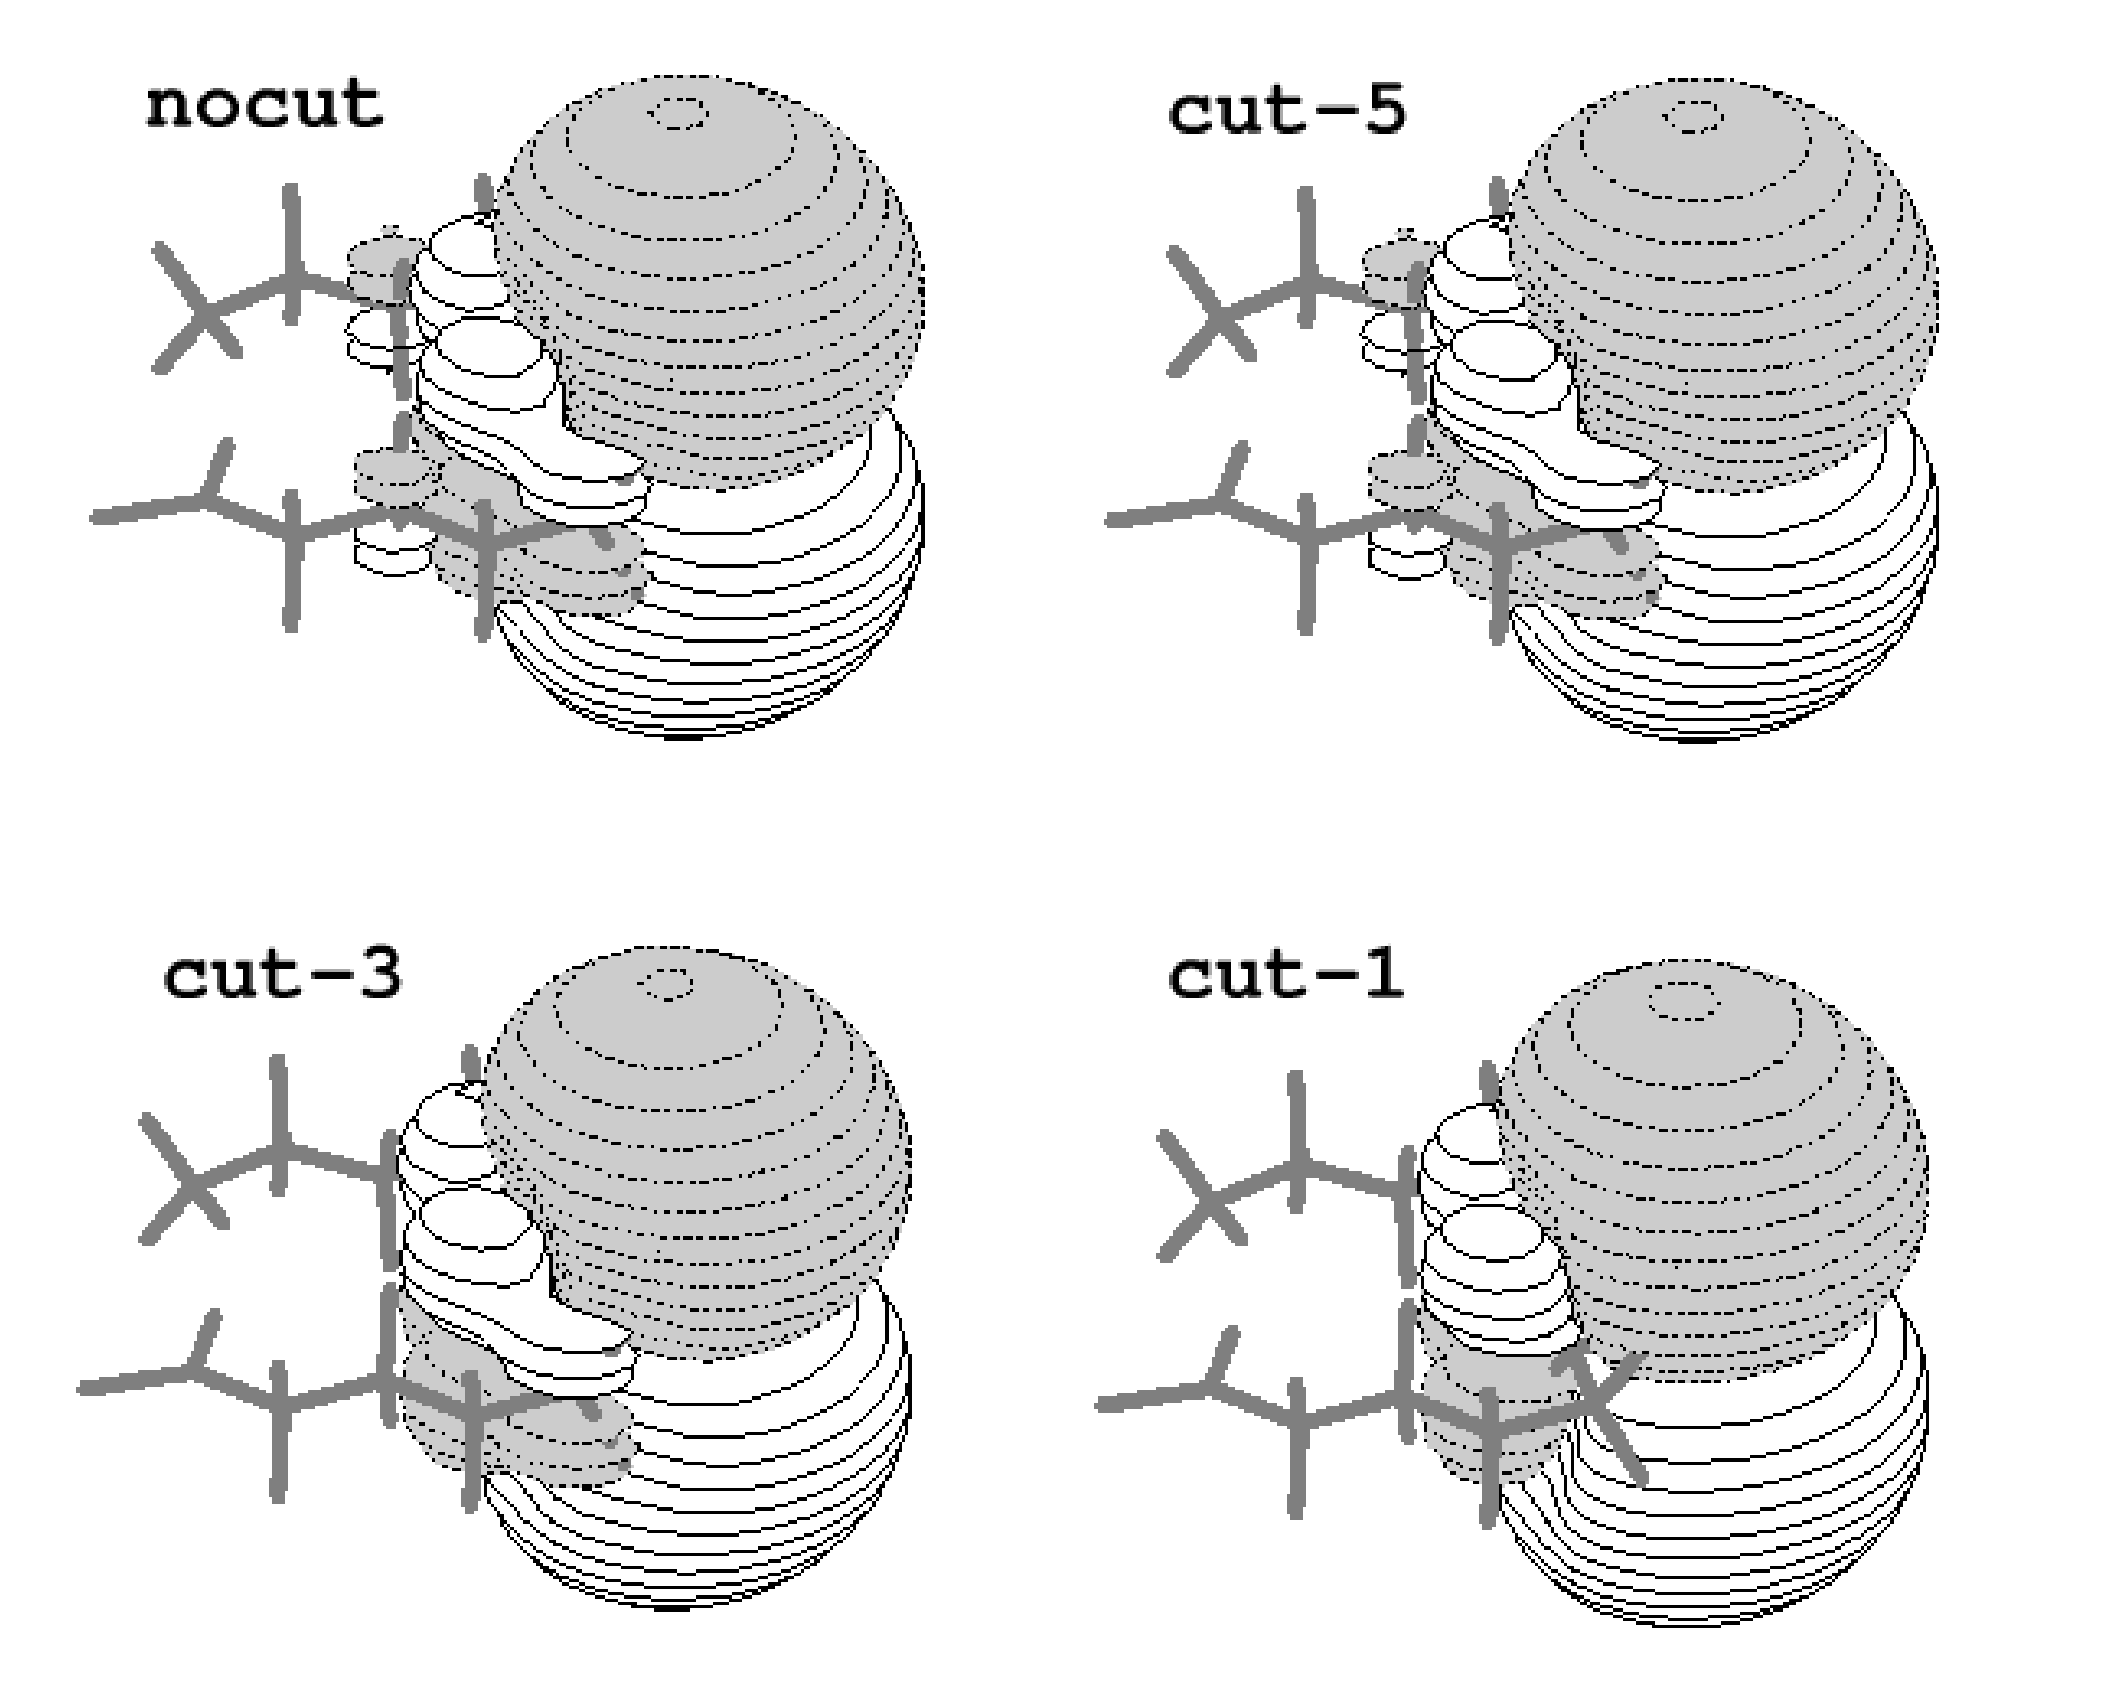
\includegraphics[width=72mm,keepaspectratio]{02_localization/images/7Z-orbitals.eps}
\caption{\footnotesize The $\pi$ orbital representation with respect to different cut strategies at frz-1
freeze strategy. }
\label{fig:7Z-orbitals}
\end{center}
\end{figure}
\end{center}



The improvements in timings are presented as an example in Tab. \ref{tbl:timings},
applied to the (7Z)-13 ammoniotridec-7-enoate with the CAS 2/2 space.

As can be seen, performing the integral evaluation on the reduced
system is a lightweight process.
Nocut evaluations have a value of zero for the reduced system. The integral
evaluation on the complete system can be used in this case, saving the cost
of a new evaluation.

The remaining steps are quite fast, but the best compromise between result
quality and time is for the frz-3/cut-3 evaluation.
In this case a reduction of the time needed to perform the optimization is
counterbalanced by the need of an integral evaluation on the small system,
but the difference between the frz-3/cut-3 and the frz-3/nocut becomes
dramatic when working on systems larger than the presented ones, which are
the final targets of this technique.

\begin{center}
\begin{table}[ht]
\footnotesize
\begin{center}
\begin{tabular}{lcccccc}
\hline
				&	seward-large	&	seward-small		&	large	& small	&	CAS+S	&	total \\
\hline
nofrz/nocut		&	1009			&			0			&	50		&	39		&	1062	&	2160 \\
frz-5/nocut		&	1009			&			0			&	50		&	19		&	355		&	1433 \\
frz-5/cut-5		&	1009			&			433			&	50		&	6		&	225		&	1723 \\
frz-3/nocut		&	1009			&			0			&	50		&	7		&	184		&	1250 \\
frz-3/cut-3		&	1009			&			100			&	50		&	1		&	99		&	1259 \\
frz-1/nocut		&	1009			&			0			&	50		&	2		&	43		&	1104 \\
frz-1/cut-1		&	1009			&			8			&	50		&	0		&	18		&	1085 \\
\hline
\end{tabular}
\end{center}
\caption{\footnotesize Timings (in seconds) for evaluations performed on (7Z)-13
ammoniotridec-7-enoate, against different freeze and cut strategies. Test
performed on Intel dual Xeon 2.8 GHz 2 GB RAM. ``seward-large'' and ``seward-small''
are the timings for the AO integral evaluation. ``large'' and ``small'' columns
represents the timings needed for the creation of the transformed integrals
which will seed the first iteration. ``CAS+S'' column reports the timings for
the complete iterative procedure up to the convergence.}
\label{tbl:timings}
\end{table}
\end{center}



\subsection{C$_{13}$ polyenal}

A second test was performed on the highly conjugated C$_{13}$ polyenal

\begin{center}
\begin{figure}[ht]
\begin{center}

\includegraphics[width=10cm]{02_localization/images/C13-molecule.eps}
\end{center}
\caption{\footnotesize The C$_{13}$ transoid polyenal molecule. }
\label{fig:C13-molecule}
\end{figure}
\end{center}

\vspace{-5mm}
Applications of the localization technique on polyenals have been performed
\cite{mp-101-1389-2003,cpl-372-22-2003,ijqc-97-688-2004}.
This class of molecules is of particular interest due to their role in
photobiology as chromophores \cite{jacs-118-7790-1996}.
Moreover, they are excellent model systems for studying
the interaction between the $\pi$ system of the carbonyl group and the
$\pi$ system of the unsaturated chain \cite{tetrahedron-34-3591-1978}. 

The cisoid-transoid energy difference for the aldehydic group has been
studied, by rotating by 180 degrees the C-C single bond. This evaluation
should be very weakly affected by the length of the polyene chain. The
distances (in $\mbox{{\AA}ngstrom}$) are r(C=O)=1.220, r(C-C)=1.450,
r(C=C)=1.350, r(C-H)=1.100.  All angles are 120 degrees.  The cut and freeze
denomination follows the analogy with shorter chain polyenals, as depicted
in Fig.~\ref{fig:C13-selection}.

\begin{center}
\begin{figure}[h!]
\begin{center}
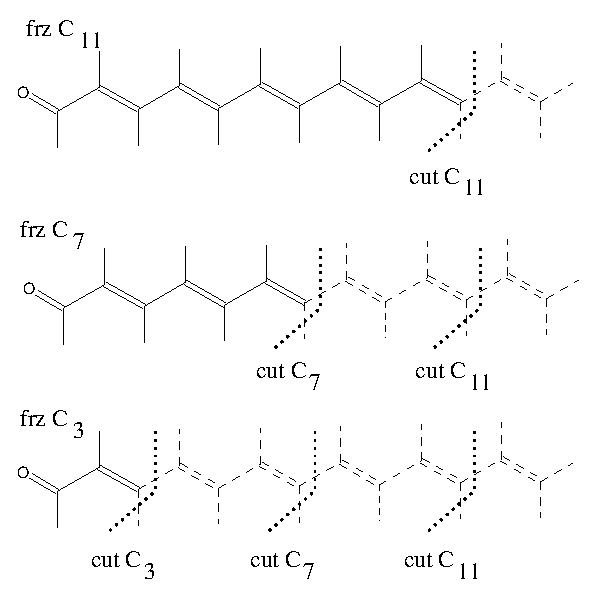
\includegraphics[width=8cm,keepaspectratio]{02_localization/images/C13-selection.eps}
\end{center}
\caption{\footnotesize C$_{13}$ polyenal molecule. Freeze and cut strategy
and labels follow the analogy with shorter chain polyenals. Localized
orbitals expressed on atoms of the dashed line framework are frozen.
Dotted lines depict the cut seam.  }
\label{fig:C13-selection}
\end{figure}
\end{center}


Two basis sets have been used: a minimal basis of type ANO-1 with $2s1p$
contraction for C and O, and a $1s$ contraction for hydrogen atoms
(hereafter named ANO-small), and a larger one ANO-1 with $3s2p$ contraction
for C and O, and a $2s$ contraction for hydrogens (ANO-large). As in the
previous case, the $1s$ core orbitals for carbon and oxygen atoms have been
frozen regardless of the freezing strategy.

Two CAS spaces have been considered. The first one, named CAS-A, contains
two electrons in the $\pi$/$\pi^{*}$ orbitals of the carbonyl group. The
second active space, named CAS-B, is defined as the previous one, further
extended with the inclusion of two additional electrons and the
$\pi$/$\pi^{*}$ orbitals from the double bond near the carbonyl. 

A preliminary evaluation with the ANO-small basis set and the CAS-A active
space has been performed on smaller polyenals, obtained by replacing the
removed part of the molecule with a hydrogen atom. The obtained results are
presented in Tab.~\ref{tbl:smaller-poly}.

\begin{center}
\begin{table}[ht]
\begin{center}
\footnotesize
\begin{tabular*}{0.75\textwidth}{l@{\hspace*{40mm}}ccc}
\hline
      	&    cisoid	&   transoid	  & diff	 \\
\hline
C$_{3}$ 	& -190.457653  	&	-190.460042   &	1.4981    \\
C$_{7}$ 	& -343.919126  	&	-343.921129   &	1.2563    \\
C$_{11}$	& -497.381057   &	-497.383042   &	1.2446    \\
C$_{13}$	& -574.112029   &	-574.114015   & 1.2453    \\
\hline
\end{tabular*}
\end{center}
\caption{\footnotesize CAS+S energy (Hartree) and difference (kcal/mol) between cisoid and
transoid complete structure for smaller polyenals, using the CAS-A active
space and the ANO-small basis set.}
\label{tbl:smaller-poly}
\end{table}
\end{center}


Tab. \ref{tbl:C13-cis-trans-diff} shows the absolute values for the CAS-A
with ANO-small basis set. Values are well reproduced, except when the cut is
near the frozen/non-frozen seam. This confirms the preceding statement
about this behavior. Also, the relative energies behave as expected. Again,
we can see that in the most pronounced Freeze-and-Cut strategy the results
are poor even in the relative energy.

Evaluation with the larger CAS-B (Tab.~\ref{tbl:C13-cis-trans-diff-casb})
and with the larger ANO-large basis set
(Tab.~\ref{tbl:C13-cis-trans-diff-ano-large}) show the same behavior.

Finally Fig. \ref{fig:C13-orbitals} shows the $\pi$ orbital for different cut
strategies, on the cisoid structure. Again, the Molden contour factor was
0.002, and the same behavior reported for the (7Z)-13 ammoniotridec-7-enoate
can be appreciated.  The cut-C11 strategy does not change the orbital in a
significant way, due to the graphically negligible expression of the
orthogonalization tail of the orbital on the removed part.  The other
strategies progressively restrict the orbital into the preserved part of
the polyenal.

\begin{center}
\begin{table}[ht]
\footnotesize
\begin{center}
\begin{tabular}{lcccc}
\hline                                                      
        &    nofrz       &    frz C$_{11}$      &   frz C$_{7}$        &   frz
C$_{3}$      \\
\hline                                                      
			&	\multicolumn{4}{c}{Cisoid} \\
nocut	&  -574.112029   &  -574.112025    &  -574.111981   & -574.110699   \\
cut C$_{11}$	&             	 &  -573.831612    &  -574.110383   & -574.110600   \\
cut C$_{7}$	&             	 &                 &  -573.826403   & -574.108770   \\
cut C$_{3}$	&             	 &             	  &                & -573.837474  	\\
			&	\multicolumn{4}{c}{Transoid} \\
nocut		&	-574.114015  	&	-574.114009  	&	-574.113945  	& -574.112686   \\
cut C$_{11}$&	             	&	-573.833584  	&	-574.112346  	& -574.112589   \\
cut C$_{7}$	&					&					&	-573.828399  	& -574.110797   \\
cut C$_{3}$	&					&					&					& -573.838137  	\\
			&	\multicolumn{4}{c}{Diff} \\
nocut			& 1.2453    &	1.2438    	&	1.2367    	&	1.2461    \\
cut C$_{11}$	&			&  	1.2367    	&	1.2314    	&	1.2474    \\
cut C$_{7}$		&			&				&  	1.2513    	&	1.2708    \\
cut C$_{3}$		&			&				&				&  	0.4161    \\
\hline
\end{tabular}
\end{center}
\caption{\footnotesize CAS+S absolute energies (Hartree) and energy
difference (kcal/mol) between cisoid and transoid C$_{13}$ polyenal using
the CAS-A active space and the ANO-small basis set, with respect to
different freeze and cut strategies.}
\label{tbl:C13-cis-trans-diff}
\end{table}
\end{center}

\begin{center}
\begin{table}[!ht]
\footnotesize
\begin{center}
\begin{tabular}{lcccc}
\hline
       &    nofrz       &    frz C$_{11}$      &   frz C$_{7}$        &   frz
C$_{3}$      \\
\hline                                                      
			&	\multicolumn{4}{c}{Cisoid} \\
nocut		&  -574.173041   &  -574.172995    	&  -574.172423   & -574.158115   \\
cut C$_{11}$&             	 &  -573.892623    	&  -574.170812   & -574.157975   \\
cut C$_{7}$	&             	 &                	&  -573.887517   & -574.156091   \\
cut C$_{3}$	&             	 &					&                & -573.889043  	\\
			&	\multicolumn{4}{c}{Transoid} \\
nocut		&	-574.174560  	&	-574.174521  	&	-574.174006  	& -574.160153   \\
cut C$_{11}$&	             	&	-573.894131  	&	-574.172393  	& -574.160015   \\
cut C$_{7}$	&					&					&	-573.889012  	& -574.158166   \\
cut C$_{3}$	&					&					&					& -573.888923  	\\
			&	\multicolumn{4}{c}{Diff} \\
nocut			& 0.9522    &	0.9567    	&	0.9919    	&	1.2776    \\
cut C$_{11}$	&			&  	0.9459    	&	0.9916    	&	1.2795    \\
cut C$_{7}$		&			&				&  	0.9378    	&	1.3015    \\
cut C$_{3}$		&			&				&				&  -0.0756    \\
\hline
\end{tabular}
\end{center}
\caption{\footnotesize CAS+S absolute energies and energy difference
(kcal/mol) between cisoid and transoid C$_{13}$ polyenal using the CAS-B
active space and the ANO-small basis set with respect to different freeze
and cut strategies.}
\label{tbl:C13-cis-trans-diff-casb}
\end{table}
\end{center}


\begin{center}
\begin{table}[!ht]
\footnotesize
\begin{center}
\begin{tabular}{lcccc}
\hline                                                      
        &    nofrz       &    frz C$_{11}$      &   frz C$_{7}$        &   frz C$_{3}$      \\
\hline                                                      
			&	\multicolumn{4}{c}{Cisoid} \\
nocut		&  -575.112195   &  -575.112194    	&  -575.112159   & -575.111082   \\
cut C$_{11}$&             	 &  -574.845588    	&  -575.108852   & -575.110774   \\
cut C$_{7}$	&             	 &                	&  -574.833700   & -575.106924   \\
cut C$_{3}$	&             	 &					&                & -574.850622  	\\
			&	\multicolumn{4}{c}{Transoid} \\
nocut		&	-575.115498  	&	-575.115500  	&	-575.115451  	& -575.114549   \\
cut C$_{11}$&	             	&	-574.848881  	&	-575.112168  	& -575.114263   \\
cut C$_{7}$	&					&					&	-574.837108  	& -575.110644   \\
cut C$_{3}$	&					&					&					& -574.849650  	\\
			&	\multicolumn{4}{c}{Diff} \\
nocut			& 2.0716    &	2.0738    	&	2.0644    	&	2.1742    \\
cut C$_{11}$	&			&  	2.0652     	&	2.0792    	&	2.1877    \\
cut C$_{7}$		&			&				&  	2.1369    	&	2.3328    \\
cut C$_{3}$		&			&				&				&  -0.6100    \\
\hline
\end{tabular}
\end{center}
\caption{\footnotesize CAS+S absolute energies and energy difference
(kcal/mol) between cisoid and transoid C$_{13}$ polyenal using the CAS-A
active space and the ANO-large basis set with respect to different freeze
and cut strategies.}
\label{tbl:C13-cis-trans-diff-ano-large}
\end{table}
\end{center}


\begin{figure}[!ht]
\begin{center}
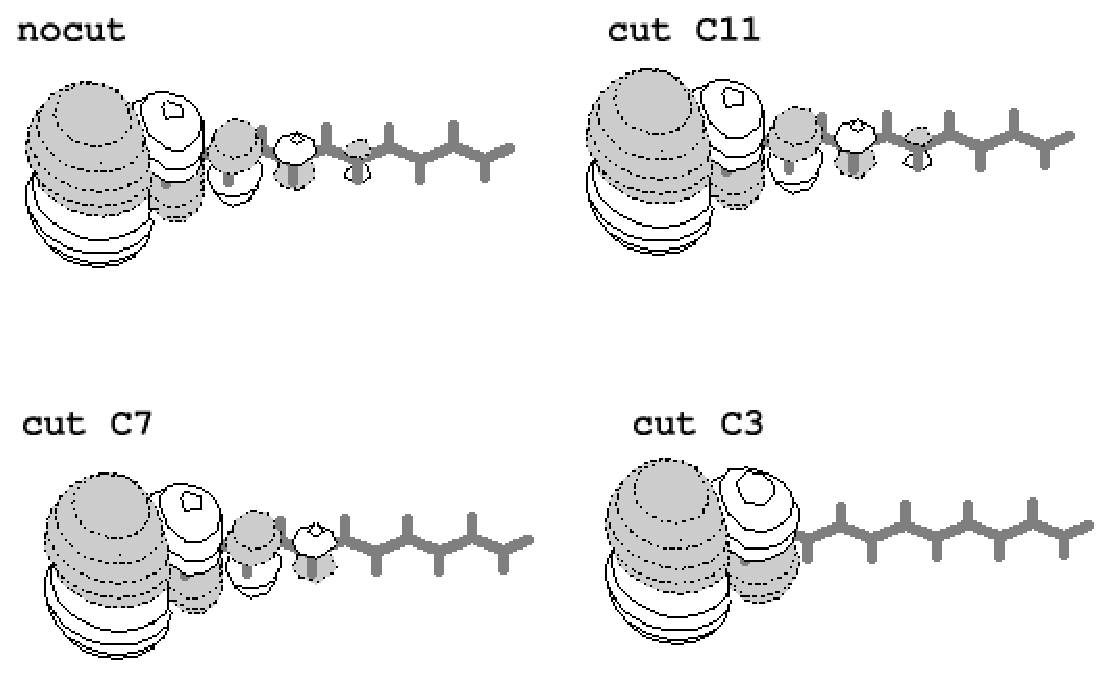
\includegraphics[width=8cm]{02_localization/images/C13-orbitals.eps}
\end{center}
\caption{\footnotesize The $\pi$ orbital for the C$_{13}$ cisoid polyenal with respect to
different cut strategies at frz-C$_{3}$ freeze strategy. The Molden contour factor for
the plot is 0.002. The progressive neglect of the orbital expression on
cut atoms can be appreciated.
}
\label{fig:C13-orbitals}
\end{figure}



\clearpage

\newpage
\subsection{Acetone + Water}

To gain better insights about the sensibility of the technique with respect
to the basis set, another test has been performed with the acetone molecule
surrounded by six water molecules. Two molecules are directly coordinated to
the carbonyl oxygen, while the remaining four coordinate the first
two molecules.

\begin{figure}[ht]
\begin{center}
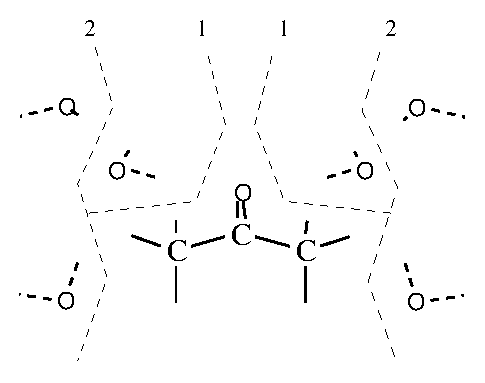
\includegraphics[width=10cm,keepaspectratio]{02_localization/images/acetone-water-frzcut-schema.eps}
\caption{\footnotesize Scheme for freeze and cut of the acetone + 6 H$_2$O
system. Surrounding water molecules have been completely frozen, and two cut
seams have been chosen to remove these molecules completely (seam ``1'') or
partially (seam ``2''). }
\label{fig:acetone-water-frzcut-schema}
\end{center}
\end{figure}

\vspace{-5mm}
The freeze and cut scheme focuses on a full freezing of the water molecules.
Two cut levels have been implemented: the first level completely removes the
water system, and the second level preserves only the two carbonyl-coordinated molecules.

The active space included five orbitals (the oxygen $n_y$ lone pair, and
carbonyl $\pi$, $\pi^{*}$, $\sigma$ and $\sigma^{*}$ orbitals) with six
active electrons. A state average optimization involving the ground state
and the $n \rightarrow \pi^{*}$ has been performed to evaluate this vertical
transition energy.

Two ANO-1 basis sets contractions have been used: the minimal set
C,O[$2s1p$], H[$1s$], hereafter called Bas-A, and an extended set
C,O[$3s2p1d$], H[$2s1p$] (Bas-B). An additional set named Bas-C is further
enriched up to C,O[$4s3p1d$], H[$2s1p$], and has been used on a smaller
system made up of the acetone molecule and two water molecules.


Tab. \ref{tbl:acetone_basis} reports the values obtained. 
The behavior of the absolute energies is as expected by previous experience:
when the cut seam is too near to the optimizable region, a difference in
absolute energy is obtained. 
\begin{center}
\begin{table}[ht]
\begin{center}
\footnotesize
\begin{tabular*}{0.80\textwidth}{l@{\hspace*{10mm}}ccc}
\hline                                                      
        &    GS       &  $n \rightarrow \pi^{*}$     &   Diff.     \\
\hline                                                      
       \multicolumn{4}{c}{Bas-A} \\
nofrz/nocut	&  -647.40071625 & -647.24175725 & 4.33 \\
frz-1/nocut &  -647.39584150 & -647.23311463 & 4.43 \\
frz-1/cut-2 &  -647.34998205 & -647.18699040 & 4.43 \\
frz-1/cut-1 &  -647.28453399 & -647.11306062 & 4.67 \\
        \multicolumn{4}{c}{Bas-B} \\
frz-1/nocut &  -648.52624523 & -648.34449917 & 4.94 \\
frz-1/cut-2 &  -645.78542705 & -645.59889274 & 5.07 \\
frz-1/cut-1 &  -644.71575515 & -644.51034075 & 5.59 \\
       \multicolumn{4}{c}{Bas-B non-ortho}  \\
frz-1/cut-2 &  -648.70019443 & -648.52408727 & 4.79 \\
frz-1/cut-1 &  -648.93490599 & -648.73207516 & 5.52 \\
\hline
\end{tabular*}
\end{center}
\caption{\footnotesize CAS+S absolute energies (Hartree) and energy
difference (eV) between ground state and $n \rightarrow \pi^{*}$ state of
acetone + 6 H$_2$O, using the minimal Bas-A basis set and the extended basis
set Bas-B (see text). Bas-B non-ortho refers to an evaluation with 
non-orthonormal orbitals.}
\label{tbl:acetone_basis}
\end{table}
\end{center}


The relative behavior, however, is poorly
affected.  When a large basis set is used, the absolute energy drift is
strongly increased. The larger Bas-B basis set produces a very steep
variation compared to the minimal Bas-A. 

\begin{figure}[ht]
\begin{center}
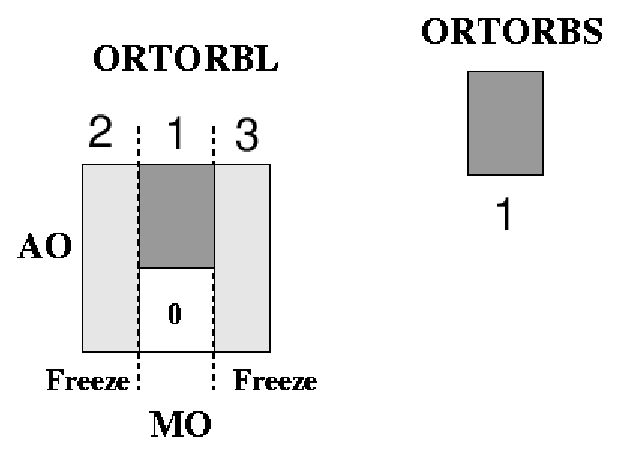
\includegraphics[width=7cm,keepaspectratio]{02_localization/images/matrix-2.eps}
\caption{\footnotesize A visual representation of the hierarchical
orthonormalization performed on the orbitals. The non-frozen orbitals
(marked with ``1'' in figure) are orthonormalized among themselves.
Then, frozen core orbitals (marked with ``2'' in figure) are orthonormalized
among themselves and against the non-frozen ones. Finally, the frozen
virtual orbitals (marked with ``3'') are orthonormalized against ``1'' and ``2''.
}
\label{fig:matrix-2}
\end{center}
\end{figure}



An additional effect must be considered responsible of the reported
behavior.  Further investigations, performed with the smaller system acetone
+ 2 H$_2$O, revealed a problem related to the molecular orbital hierarchical
orthonormalization (Fig.~\ref{fig:matrix-2}). After the cut action,
orbitals are no longer orthonormal, and the orthonormalization procedure
aims at restoring this orthonormality. 

The first class of orbitals performing the orthonormalization is the
non-frozen zone (marked ``1'' in Fig.~\ref{fig:matrix-2}) which remains
described in the smaller AO space. This class must be treated first, in
order to preserve itself inside this restricted space.

The second class is the frozen core orbitals class (marked ``2'' in
Fig.~\ref{fig:matrix-2}). When this class is orthonormalized with respect to
the first one, orthonormalization tails are produced, effectively changing
the core orbitals. The weight and spatial distribution of these tails is
bound to the atomic basis set used to describe the molecular system,
therefore larger basis sets produce stronger effects.

This situation is different from the previously reported phenomenon in
7Z-13 ammoniotridec-7-enoate in the frz-3/cut-3 analysis, where hydrogen
atoms were removed from non-frozen orbitals. In the current case, frozen
orbitals are modified due to orthonormality needs, which impose tails toward
nearby atoms. These tails introduce an artificial charge shift toward these
atoms, and in particular those involved in the physical process under
study, resulting in convergence problems or a high energy drift. The process
sometimes makes impossible for the evaluation to converge.

Molden plots have been performed on the smaller system with only two water
molecules. The contour factor is 0.03. Fig.~\ref{fig:acetone_tails} shows a
clear difference between the water OH bond with the Bas-C contraction and
the Bas-A contraction.

\begin{figure}[ht]
\begin{center}
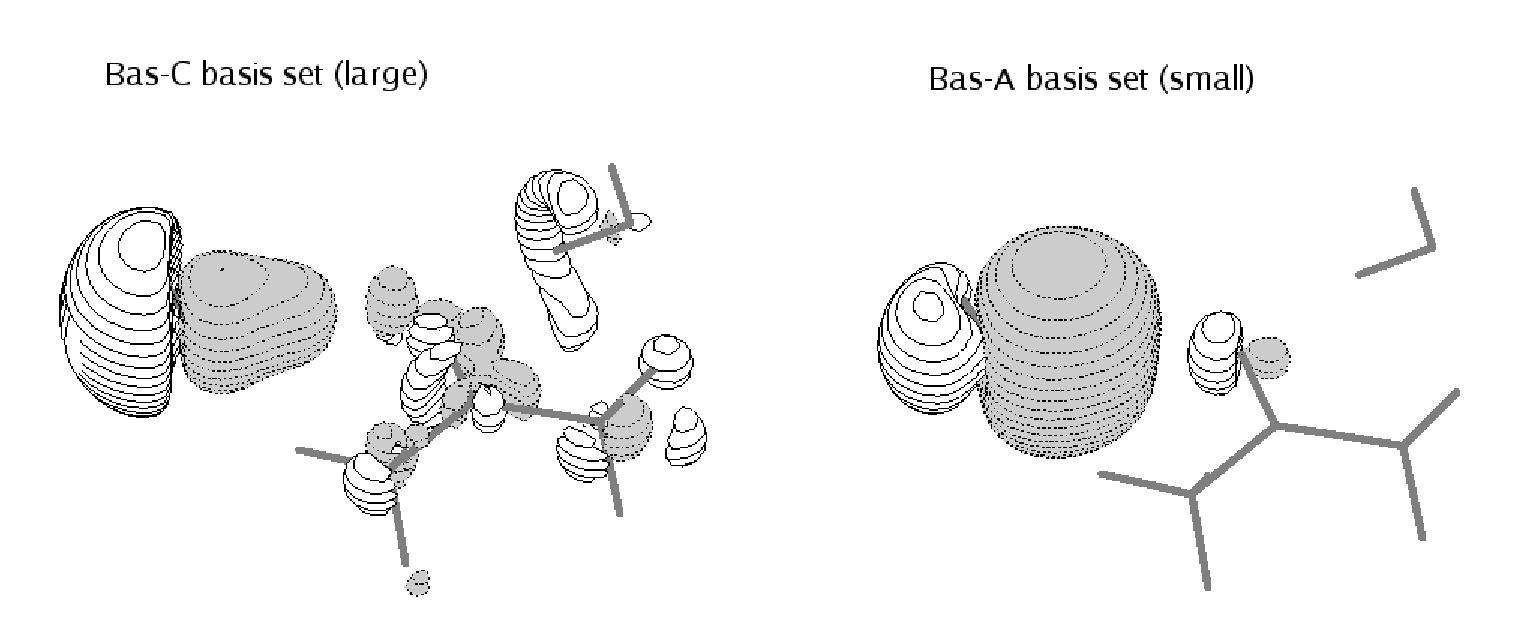
\includegraphics[width=12cm,keepaspectratio]{02_localization/images/acetone_tails.eps}
\caption{\footnotesize The water OH bond on the small acetone +
2H$_2$O system, using the large basis set Bas-C and the small Bas-A. The
difference in spatial distribution of the orthonormalization tails is
clearly visible. }
\label{fig:acetone_tails}
\end{center}
\end{figure}

\vspace{-5mm}
The nature of this problem is independent of the frozen spacer between the
removed zone and the non-frozen zone, but related to the frozen/non-frozen
seam. The problem do not arise when cut is not performed, and consequently
the resulting orbitals do not incur in orthonormalization. 

At first glance, a possible solution is to keep the frozen/non-frozen seam
as much far as possible from the region interested in the chemical
phenomenon, leading to absolute energy drifts but prevent tails to
act on the active space. However, this goes in the direction of incrementing
the computational cost of the final evaluation, enlarging the non-frozen
zone in a large basis regime.

Another possible solution has been attempted working with a non-orthonormal
basis set. Frozen orbitals are not orthonormalized with respect to the
non-frozen ones, and the results obtained (Tab.~\ref{tbl:acetone_basis}
non-ortho) show a cleaner behavior. However, it must be pointed out that this
procedure is not strictly formal under the assumptions made for the current
theoretical deployment, and the convergence is very slow. An improvement in
the theoretical asset is needed to formally work around this problem.

\section{Conclusions}

The Freeze-and-Cut technique has proved its usefulness in optimizing local
orbitals at CASSCF or quasi-CASSCF level. It combines the freeze of the
molecular orbitals that are not relevant for the phenomenon under study, and
the cut of those atoms that are not needed to describe the optimized
orbitals.

Different levels of theory can be used for the molecular framework and the
physically interesting region of the system.  The presented test cases
demonstrate the ability of the method to give essentially the same results
as a localized CASSCF calculation on the complete system, with a
significant reduction of the computational cost.

Two problems must be kept into account in order to obtain reliable CASSCF
energies: the first problem involves the tails of the unfrozen orbitals,
which can have a significant delocalization on the nearest neighbor atoms.
The projection of the unfrozen orbitals into a restricted set of atoms has
the effect of rising the absolute energy, but the relative energies seems to
be poorly affected. 

The second problem is relative to the methodological need to reorthonormalize
the frozen orbitals set after the cut is performed. This can introduce artificial
tails which can create instability when occurring near the active
orbitals. Both effects depend on the atomic basis set spatial distribution.

To face these problems, a general strategy can be devised:
\begin{itemize}
\item reduce the cut out of the unfrozen orbitals, setting the cut seam
far from the unfrozen region. Atoms which are geometrically very distant
from the unfrozen set can be usually cut out safely
\item reduce the influence of the frozen orbitals orthonormalization tails 
on the chemically active region (usually, the active orbitals).  To minimize
this effect, a sufficient spacer of unfrozen orbitals should be kept.
\end{itemize}
Further evaluations are however needed to gain detailed comprehension of
this strategy.

